\section{Appendix\label{sec:appendix}}
\subsection{Simulation results for two clients\label{sec:2_clients}}
In the following, we report results for simulations with two clients for the four scenarios. The results are generated with individual test datasets for all clients and with a unified test dataset for all clients. The motivation behind these two approaches is explained in section \ref{sec:methodology_study_setup}.

% \subsubsection{Balanced data distribution - balanced label distribution}
\begin{figure}[!h]
    \centering
    \includegraphics[width=0.75\textwidth]{outputs/2_clients/test_set_individual/1_balanced_DD_balanced_LD/performance.png}
    \caption{AUC of scenario 1 (balanced data distribution - balanced label distribution) with two clients}
    \label{fig:auc_box_2_clients_scenario_1}
\end{figure}

\begin{table}[h]
\centering
\caption{AUC welfare gains}
\label{tab:auc_welfare}
\begin{tabular}{lrr}
\toprule
{} &  WG\_AUC\_FL\_norm [\%] &  WG\_AUC\_FL\_client\_norm [\%] \\
\midrule
client\_1 &                1.24 &                       1.15 \\
client\_2 &                0.98 &                       1.07 \\
mean     &                1.11 &                       1.11 \\
sum      &                2.22 &                       2.22 \\
\bottomrule
\end{tabular}
\end{table}


\begin{figure}[!h]
    \centering
    \includegraphics[width=0.75\textwidth]{outputs/2_clients/test_set_one/1_balanced_DD_balanced_LD/performance.png}
    \caption{AUC of scenario 1 (balanced data distribution - balanced label distribution) with two clients, unified test dataset}
    \label{fig:auc_box_2_clients_scenario_1_uni}
\end{figure}

\input{outputs/2_clients/test_set_one/1_balanced_DD_balanced_LD/auc_welfare_gains_2_clients_scenario_1_uni}

% \clearpage
% \subsubsection{Unbalanced data distribution - balanced label distribution}
\begin{figure}[htb!]
    \centering
    \includegraphics[width=0.75\textwidth]{outputs/2_clients/test_set_individual/2_unbalanced_DD_balanced_LD/performance.png}
    \caption{AUC of scenario 2 (unbalanced data distribution - balanced label distribution) with two clients}
    \label{fig:auc_box_2_clients_scenario_2}
\end{figure}

\begin{table}[h]
\centering
\caption{AUC welfare gains}
\label{tab:auc_welfare}
\begin{tabular}{lrr}
\toprule
{} &  WG\_AUC\_FL\_norm [\%] &  WG\_AUC\_FL\_client\_norm [\%] \\
\midrule
client\_1 &                0.02 &                       0.04 \\
client\_2 &                3.28 &                       3.19 \\
mean     &                1.65 &                       1.62 \\
sum      &                3.30 &                       3.23 \\
\bottomrule
\end{tabular}
\end{table}


\begin{figure}[htb!]
    \centering
    \includegraphics[width=0.75\textwidth]{outputs/2_clients/test_set_one/2_unbalanced_DD_balanced_LD/performance.png}
    \caption{AUC of scenario 2 (unbalanced data distribution - balanced label distribution) with two clients, unified test dataset}
    \label{fig:auc_box_2_clients_scenario_2_uni}
\end{figure}

\input{outputs/2_clients/test_set_one/2_unbalanced_DD_balanced_LD/auc_welfare_gains_2_clients_scenario_2_uni}
% \clearpage
% \subsubsection{Balanced data distribution - unbalanced label distribution}

\begin{figure}[htb!]
    \centering
    \includegraphics[width=0.75\textwidth]{outputs/2_clients/test_set_individual/3_balanced_DD_unbalanced_LD/performance.png}
    \caption{AUC of scenario 3 (balanced data distribution - unbalanced label distribution) with two clients}
    \label{fig:auc_box_2_clients_scenario_3}
\end{figure}

\begin{table}[h]
\centering
\caption{AUC welfare gains}
\label{tab:auc_welfare}
\begin{tabular}{lrr}
\toprule
{} &  WG\_AUC\_FL\_norm [\%] &  WG\_AUC\_FL\_client\_norm [\%] \\
\midrule
client\_1 &                1.07 &                       0.94 \\
client\_2 &                0.53 &                       0.48 \\
mean     &                0.80 &                       0.71 \\
sum      &                1.61 &                       1.42 \\
\bottomrule
\end{tabular}
\end{table}


\begin{figure}[htb!]
    \centering
    \includegraphics[width=0.75\textwidth]{outputs/2_clients/test_set_one/3_balanced_DD_unbalanced_LD/performance.png}
    \caption{AUC of scenario 3 (balanced data distribution - unbalanced label distribution) with two clients, unified test dataset}
    \label{fig:auc_box_2_clients_scenario_3_uni}
\end{figure}

\input{outputs/2_clients/test_set_one/3_balanced_DD_unbalanced_LD/auc_welfare_gains_2_clients_scenario_3_uni}
% \clearpage
% \subsubsection{Unbalanced data distribution - unbalanced label distribution}

\begin{figure}[htb!]
    \centering
    \includegraphics[width=0.75\textwidth]{outputs/2_clients/test_set_individual/4_unbalanced_DD_unbalanced_LD/performance.png}
    \caption{AUC of scenario 4 (unbalanced data distribution - unbalanced label distribution) with two clients}
    \label{fig:auc_box_2_clients_scenario_4}
\end{figure}

\begin{table}[h]
\centering
\caption{AUC welfare gains}
\label{tab:auc_welfare}
\begin{tabular}{lrr}
\toprule
{} &  WG\_AUC\_FL\_norm [\%] &  WG\_AUC\_FL\_client\_norm [\%] \\
\midrule
client\_1 &                0.51 &                       0.33 \\
client\_2 &                5.86 &                       6.06 \\
mean     &                3.18 &                       3.19 \\
sum      &                6.37 &                       6.39 \\
\bottomrule
\end{tabular}
\end{table}


\begin{figure}[htb!]
    \centering
    \includegraphics[width=0.75\textwidth]{outputs/2_clients/test_set_one/4_unbalanced_DD_unbalanced_LD/performance.png}
    \caption{AUC of scenario 4 (unbalanced data distribution - unbalanced label distribution) with two clients, unified test dataset}
    \label{fig:auc_box_2_clients_scenario_4_uni}
\end{figure}

\input{outputs/2_clients/test_set_one/4_unbalanced_DD_unbalanced_LD/auc_welfare_gains_2_clients_scenario_4_uni}
\clearpage
\subsection{Simulation results for ten clients\label{sec:10_clients}}
In the following, we report results for simulations with ten clients for the four scenarios. The results are generated with individual test datasets for all clients and with a unified test dataset for all clients. The motivation behind these two approaches is explained in section \ref{sec:methodology_study_setup}.

% \subsubsection{Balanced data distribution - balanced label distribution}
\begin{figure}[htb!]
    \centering
    \includegraphics[width=0.75\textwidth]{outputs/10_clients/test_set_individual/1_balanced_DD_balanced_LD/performance_rotated.png}
    \caption{AUC of scenario 1 (balanced data distribution - balanced label distribution) with ten clients}
    \label{fig:auc_box_10_clients_scenario_1}
\end{figure}

\input{outputs/10_clients/test_set_individual/1_balanced_DD_balanced_LD/auc_welfare_gains_10_clients_scenario_1}

\begin{figure}[htb!]
    \centering
    \includegraphics[width=0.75\textwidth]{outputs/10_clients/test_set_one/1_balanced_DD_balanced_LD/performance_rotated.png}
    \caption{AUC of scenario 1 (balanced data distribution - balanced label distribution) with ten clients, unified test dataset}
    \label{fig:auc_box_10_clients_scenario_1_uni}
\end{figure}

\input{outputs/10_clients/test_set_one/1_balanced_DD_balanced_LD/auc_welfare_gains_10_clients_scenario_1_uni}
% \clearpage
% \subsubsection{Unbalanced data distribution - balanced label distribution}

\begin{figure}[htb!]
    \centering
    \includegraphics[width=0.75\textwidth]{outputs/10_clients/test_set_individual/2_unbalanced_DD_balanced_LD/performance_rotated.png}
    \caption{AUC of scenario 2 (unbalanced data distribution - balanced label distribution) with ten clients}
    \label{fig:auc_box_10_clients_scenario_2}
\end{figure}

\input{outputs/10_clients/test_set_individual/2_unbalanced_DD_balanced_LD/auc_welfare_gains_10_clients_scenario_2}

\begin{figure}[htb!]
    \centering
    \includegraphics[width=0.75\textwidth]{outputs/10_clients/test_set_one/2_unbalanced_DD_balanced_LD/performance_rotated.png}
    \caption{AUC of scenario 2 (unbalanced data distribution - balanced label distribution) with ten clients, unified test dataset}
    \label{fig:auc_box_10_clients_scenario_2_uni}
\end{figure}

\input{outputs/10_clients/test_set_one/2_unbalanced_DD_balanced_LD/auc_welfare_gains_10_clients_scenario_2_uni}
% \clearpage
% \subsubsection{Balanced data distribution - unbalanced label distribution}

\begin{figure}[htb!]
    \centering
    \includegraphics[width=0.75\textwidth]{outputs/10_clients/test_set_individual/3_balanced_DD_unbalanced_LD/performance_rotated.png}
    \caption{AUC of scenario 3 (balanced data distribution - unbalanced label distribution) with ten clients}
    \label{fig:auc_box_10_clients_scenario_3}
\end{figure}

\input{outputs/10_clients/test_set_individual/3_balanced_DD_unbalanced_LD/auc_welfare_gains_10_clients_scenario_3}

\begin{figure}[htb!]
    \centering
    \includegraphics[width=0.75\textwidth]{outputs/10_clients/test_set_one/3_balanced_DD_unbalanced_LD/performance_rotated.png}
    \caption{AUC of scenario 3 (balanced data distribution - unbalanced label distribution) with ten clients, unified test dataset}
    \label{fig:auc_box_10_clients_scenario_3_uni}
\end{figure}

\input{outputs/10_clients/test_set_one/3_balanced_DD_unbalanced_LD/auc_welfare_gains_10_clients_scenario_3_uni}
% \clearpage
% \subsubsection{Unbalanced data distribution - unbalanced label distribution}

\begin{figure}[htb!]
    \centering
    \includegraphics[width=0.75\textwidth]{outputs/10_clients/test_set_individual/4_unbalanced_DD_unbalanced_LD/performance_rotated.png}
    \caption{AUC of scenario 4 (unbalanced data distribution - unbalanced label distribution) with ten clients}
    \label{fig:auc_box_10_clients_scenario_4}
\end{figure}

\input{outputs/10_clients/test_set_individual/4_unbalanced_DD_unbalanced_LD/auc_welfare_gains_10_clients_scenario_4}

\begin{figure}[htb!]
    \centering
    \includegraphics[width=0.75\textwidth]{outputs/10_clients/test_set_one/4_unbalanced_DD_unbalanced_LD/performance_rotated.png}
    \caption{AUC of scenario 4 (unbalanced data distribution - unbalanced label distribution) with ten clients, unified test dataset}
    \label{fig:auc_box_10_clients_scenario_4_uni}
\end{figure}

\input{outputs/10_clients/test_set_one/4_unbalanced_DD_unbalanced_LD/auc_welfare_gains_10_clients_scenario_4_uni}
